\documentclass{article}
\usepackage[UTF8]{ctex}
\usepackage{pythonhighlight}
\usepackage{markdown}
\usepackage{listings}
\lstset{
    basicstyle          =   \tt,          % 基本代码风格
    identifierstyle=\color{brown!80!black},
    keywordstyle        =   \color{purple}\bfseries,          % 关键字风格
    commentstyle        =   \rmfamily\itshape,  % 注释的风格,斜体
    stringstyle         =   \ttfamily,  % 字符串风格
    flexiblecolumns,                % 别问为什么,加上这个
    numbers             =   left,   % 行号的位置在左边
    showspaces          =   false,  % 是否显示空格,显示了有点乱,所以不现实了
    numberstyle         =   \zihao{-5}\ttfamily,    % 行号的样式,小五号,tt等宽字体
    showstringspaces    =   false,
    captionpos          =   t,      % 这段代码的名字所呈现的位置,t指的是top上面
    frame               =   lrtb,   % 显示边框
    backgroundcolor=\color[RGB]{245,245,244},
}


% Language setting
% Replace `english' with e.g. `spanish' to change the document language
\usepackage[english]{babel}
\usepackage{float}
% Set page size and margins
% Replace `letterpaper' with `a4paper' for UK/EU standard size
\usepackage[letterpaper,top=2cm,bottom=2cm,left=3cm,right=3cm,marginparwidth=1.75cm]{geometry}

% Useful packages
\usepackage{amsmath}
\usepackage{graphicx}
\usepackage[colorlinks=true, allcolors=blue]{hyperref}

\title{数逻实验报告Lab7}
\author{雷远航}

\begin{document}
    
\maketitle

\begin{abstract}
    实验项目:多路选择器设计与应用
\end{abstract}

\section{操作方法与实验步骤}

\subsection{数字选择器设计}

\subsubsection*{实验原理图绘制}
    \begin{figure}[H]
	\centering
	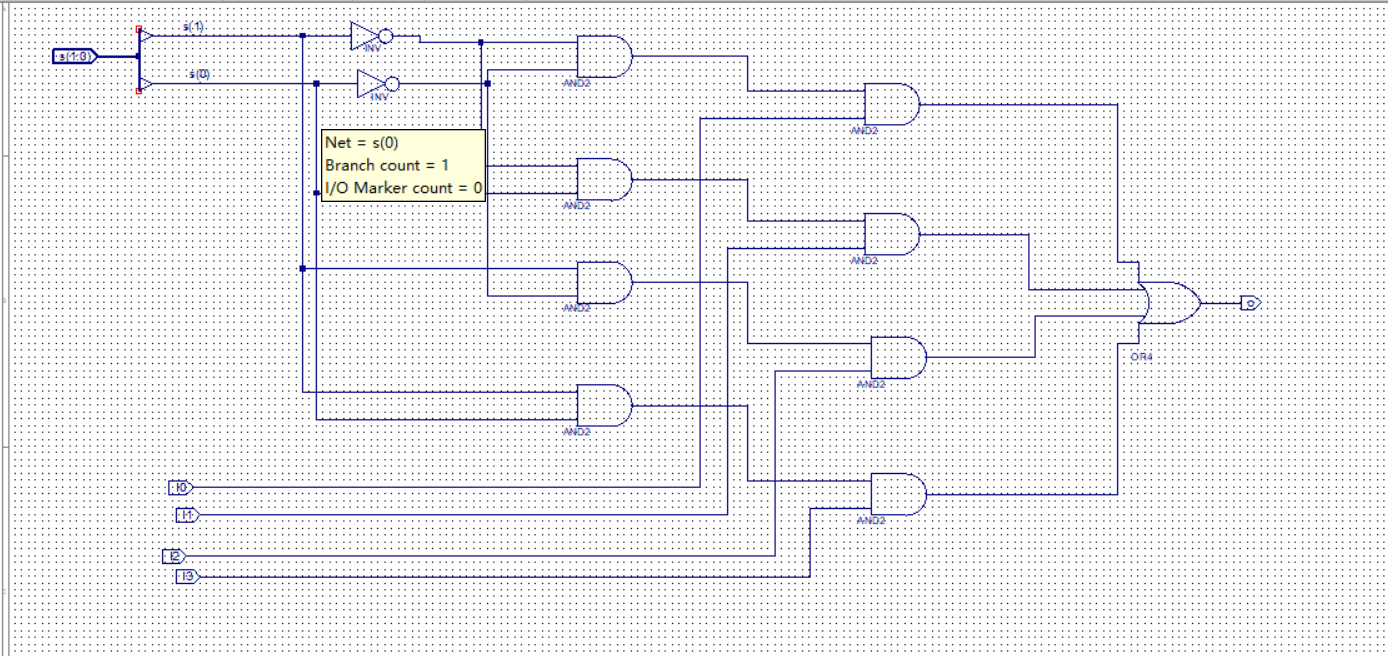
\includegraphics[width=0.9\textwidth]{lab7/5.png}
	\caption{\label{Lab7}一位MUX绘制}
	\end{figure}

    \begin{figure}[H]
    \centering
    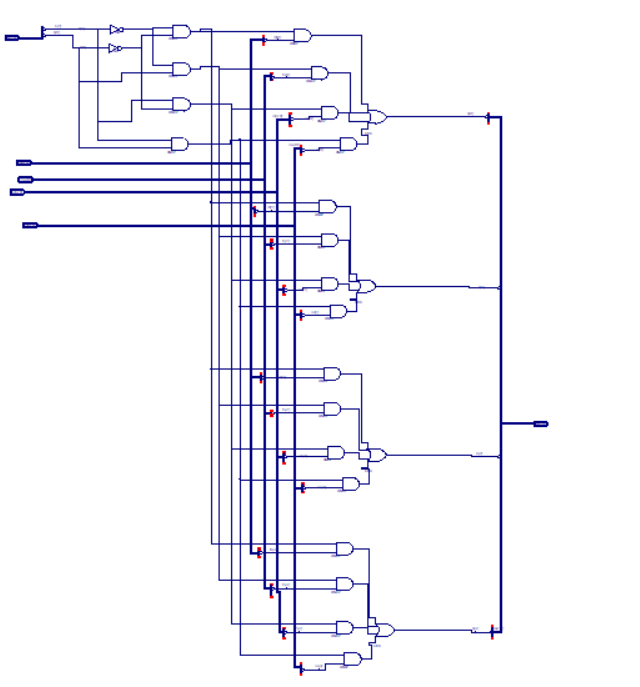
\includegraphics[width=0.9\textwidth]{lab7/2.png}
    \caption{\label{Lab7}Mux4to1b4}
    \end{figure}


\subsubsection*{进行模拟仿真}

\subsubsection*{仿真激励代码如下}
\begin{lstlisting}[language=verilog]
`timescale  1ns / 1ps

module Mux_tb();
    
    reg[3:0] I0;
    reg[3:0] I1;
    reg[3:0] I2;
    reg[3:0] I3;
    reg[1:0] s;
    wire[3:0] o;
    
    MUX m0(.I0(I0), .I1(I1), .I2(I2), .I3(I3), .s(s), .o(o));
    
    
    integer i;
    initial begin
    #50
    #5 I0 = 4'b1100;
    I1 = 4'b0011;
    I2 = 4'b1010;
    I3 = 4'b1111;
    #5
    for(i=0;i<=3;i=i+1) begin
            {s[1:1],s[0:0]} <= i;
        #50;
    end
        
    #50 I0 = 4'b0001;
    I1 = 4'b0001;
    I2 = 4'b0100;
    I3 = 4'b1000;
    #5
    
    for(i=0;i<=3;i=i+1) begin
        {s[1:1],s[0:0]} <= i;
        #50;
    end
    
        
    end
    
endmodule    
    
\end{lstlisting}







\subsection{记分板设计}

\subsubsection*{相关实验原理图绘制}

    \begin{figure}[H]
    \centering
    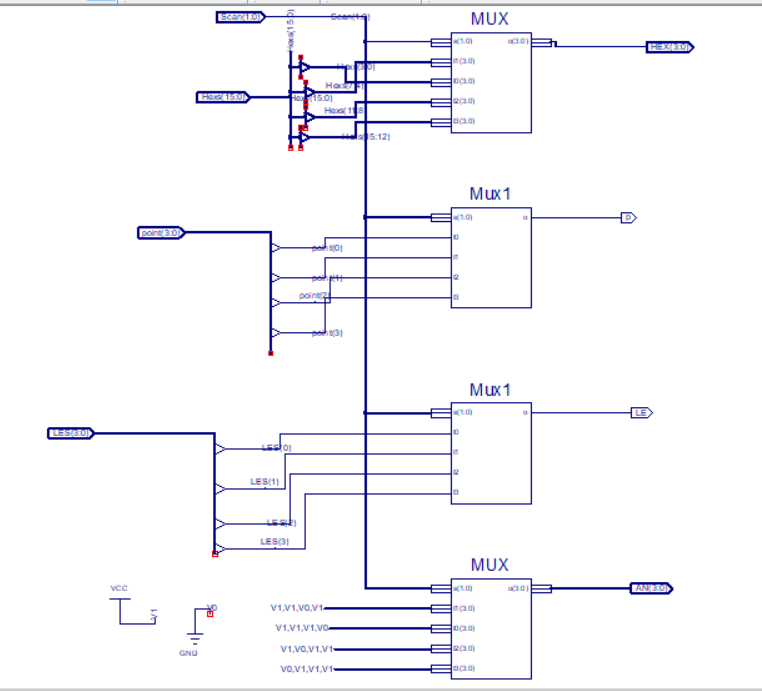
\includegraphics[width=0.9\textwidth]{lab7/7.png}
    \caption{\label{Lab7}DisPlaySync原理图绘制}
    \end{figure}

    \begin{figure}[H]
    \centering
    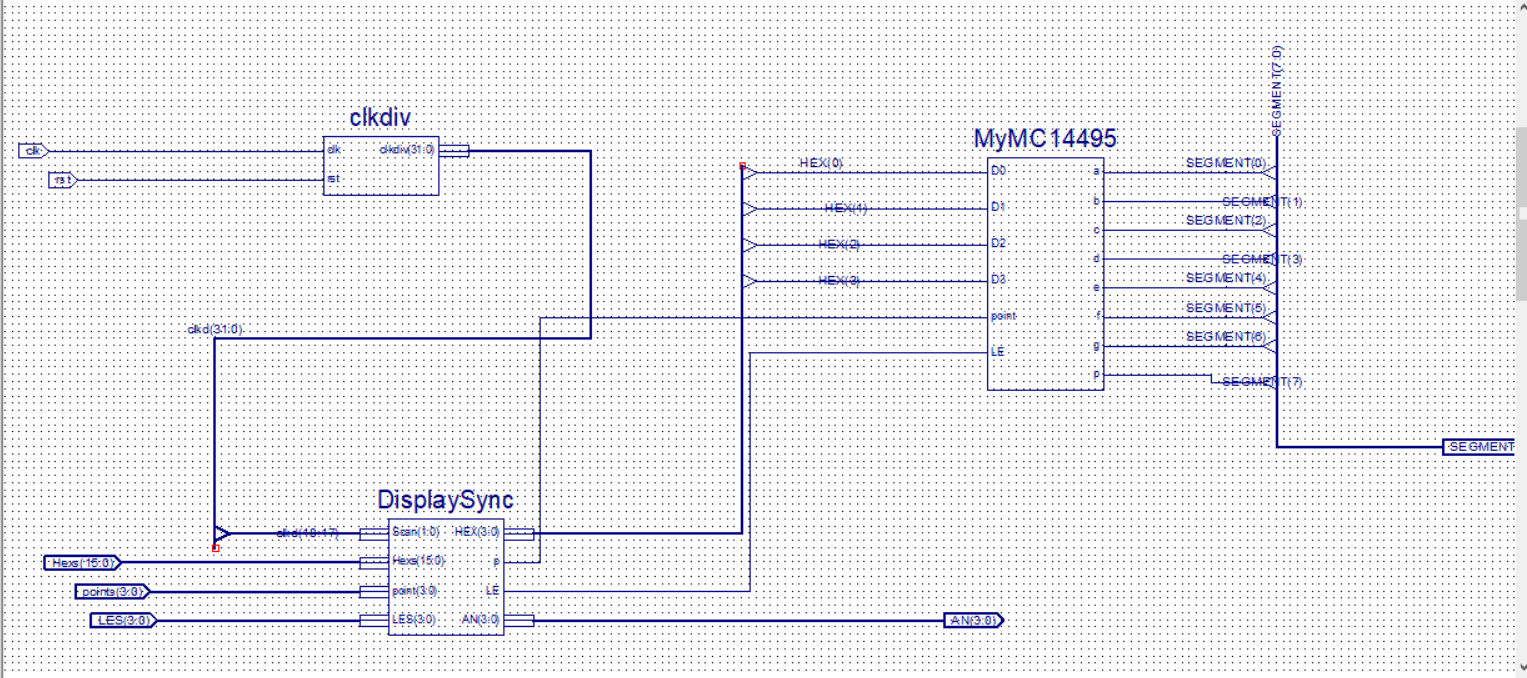
\includegraphics[width=0.9\textwidth]{lab7/6.png}
    \caption{\label{Lab7}ScoreBoard原理图绘制}
    \end{figure}

\subsubsection*{其余实验步骤}
导入clk.v 和 clk\_tb.v,进行模拟仿真
导入CreateNumber.v 和 CreateNumber\_tb.v,进行模拟仿真
导入top.v,形成完整的ScoreBoard,进行下版验证.



\section{实验结果与分析}

\subsection{数字选择器设计}

\subsubsection*{仿真波形图}
    \begin{figure}[H]
    \centering
    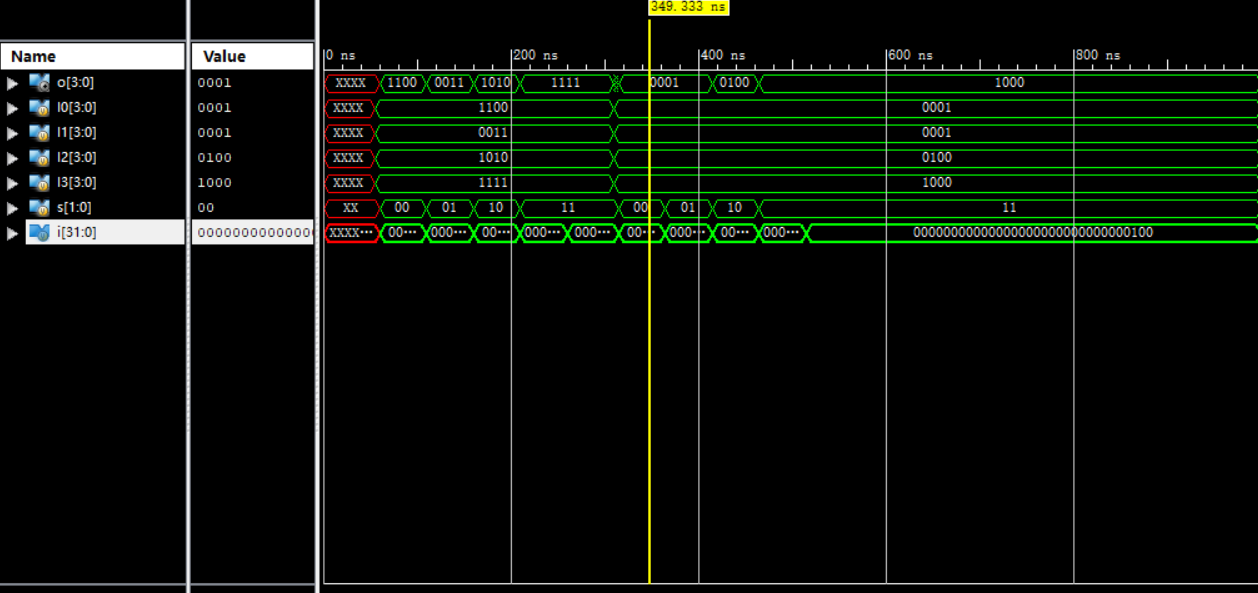
\includegraphics[width=0.8\textwidth]{lab7/1.png}
    \caption{\label{Lab7}Mux波形图}
    \end{figure}

\subsubsection*{波形图解释}
在自行书写的仿真激励代码中,第一轮对选择信号赋初值,然后通过循环使控制选择的信号从0-3(二进制形式)进行遍历,
可以看到,MUX按照控制信号,对输出的信号做出了正确的输出,可以验证所做原理图的正确性.
第二轮循环只是更改了相应的赋值,实际的过程与第一轮是类似的,可以看出最终输出的波形仍是正确的.


\subsection{记分板设计}

\subsubsection{clkdiv的波形图}

    \begin{figure}[H]
    \centering
    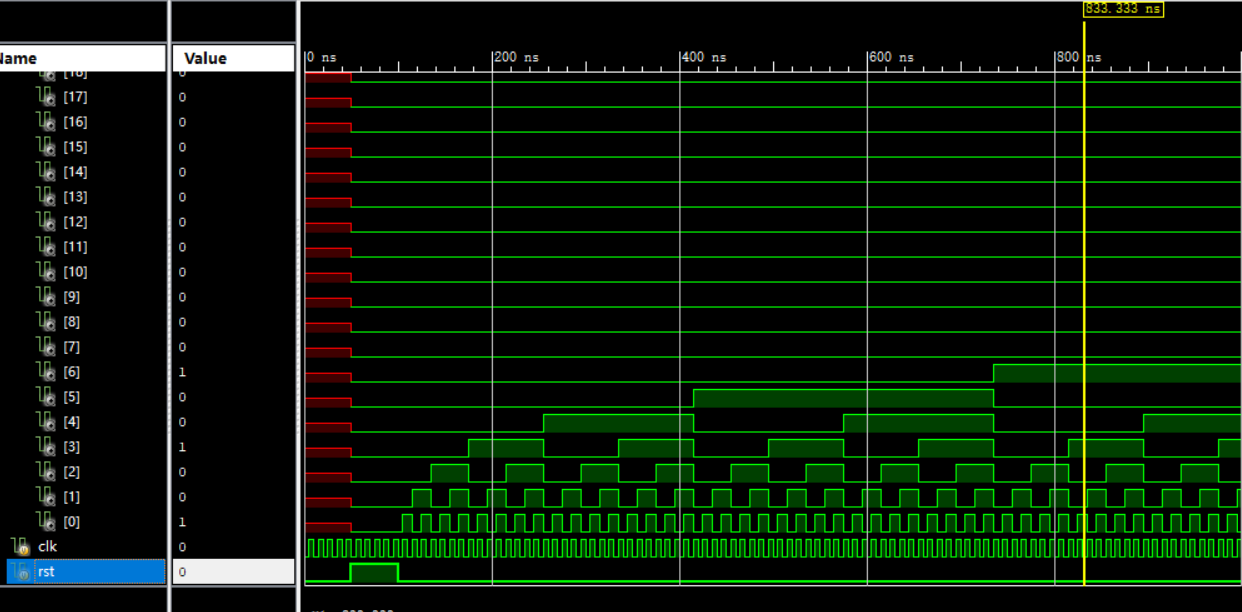
\includegraphics[width=0.9\textwidth]{lab7/3.png}
    \caption{\label{Lab7}clkdiv波形图}
    \end{figure}

\subsubsection*{clkdiv波形图解释}
根据clkdiv.v的代码实现可以看出,当rst信号处于时钟上升沿的时候,输出信号clkdiv才会发生变化,波形图与其相符合.
当clk的信号处于时钟上升沿时,clkdiv所对应的二进制数值会加1,在波形图中可以看到,信号对应的值从0开始依次递增与预期相符合.
同时很容易的发现,第[k]个对应的信号变化的周期为$2^{k+1}$个单位长度.

\subsubsection{CreateNumber的波形图}
    \begin{figure}[H]
    \centering
    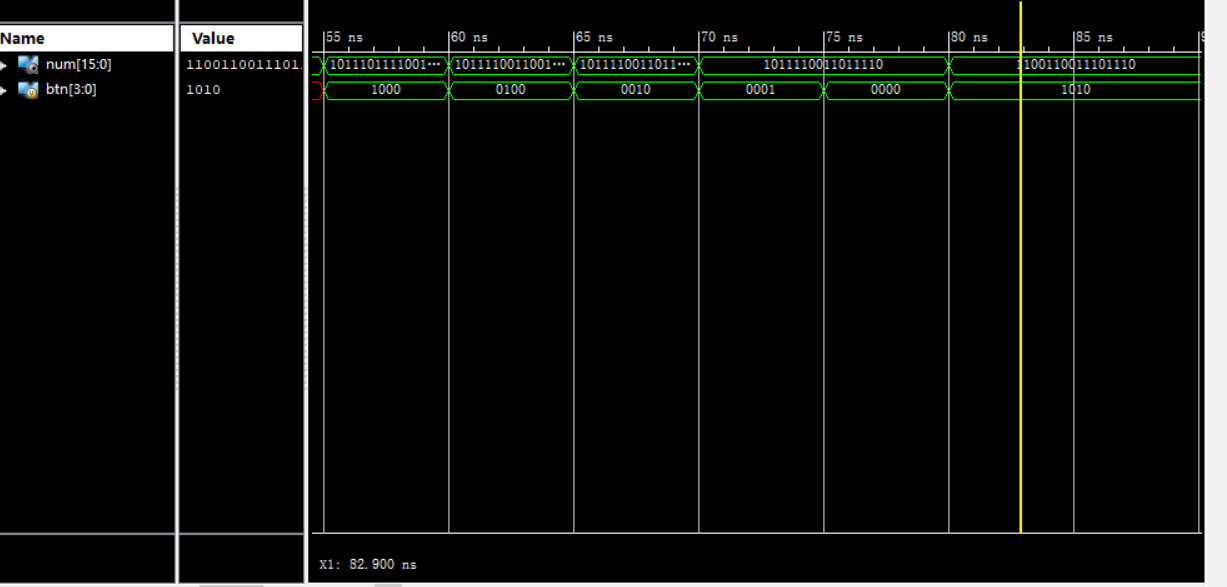
\includegraphics[width=0.9\textwidth]{lab7/8.png}
    \caption{\label{Lab7}CreateNumber波形图}
    \end{figure}

\subsubsection*{CreateNumber波形图解释}
根据CreateNumber.v可知,num[15:0]从高到低的4位,依次由 btn[i]进行控制,若btn[i]的信号为上升边沿(信号为1),则对应位的数值加一.
测试文件中首先对num赋初始值为16'b1010\_1011\_1100\_1101
在CreateNumber\_tb.v中,首先通过控制信号依次使一个,对应的四位数值加1,可以看到对应的数每次在相应的过程中值增加了1
然后设置btn信号为4'b0000,可以看到num的数值并不发生变化.
最后一次测试btn为4'b1010,因此第一个4bits数和第三个4bits数都会发生改变,波形图中的结果相符.

\subsubsection{ScoreBoard下版验证与分析}

    \begin{figure}[H]
    \centering
    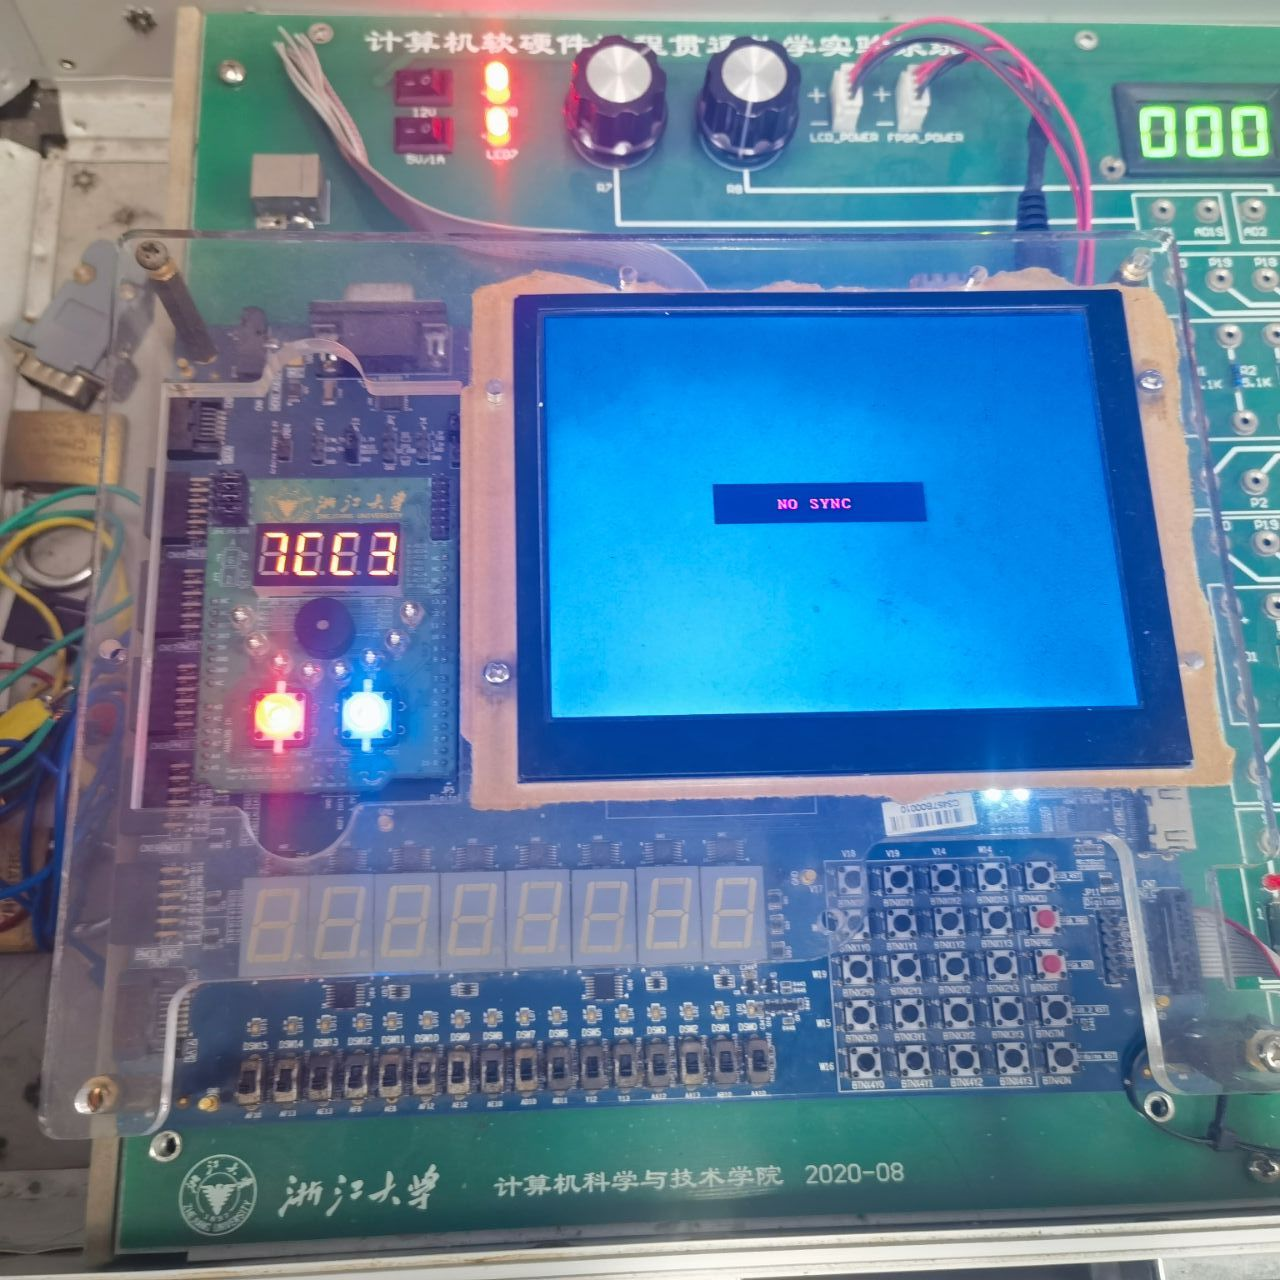
\includegraphics[width=0.4\textwidth]{lab7/9.jpg}
    \caption{\label{Lab7}ScoreBoard下版验证}
    \end{figure}

    \begin{figure}[H]
    \centering
    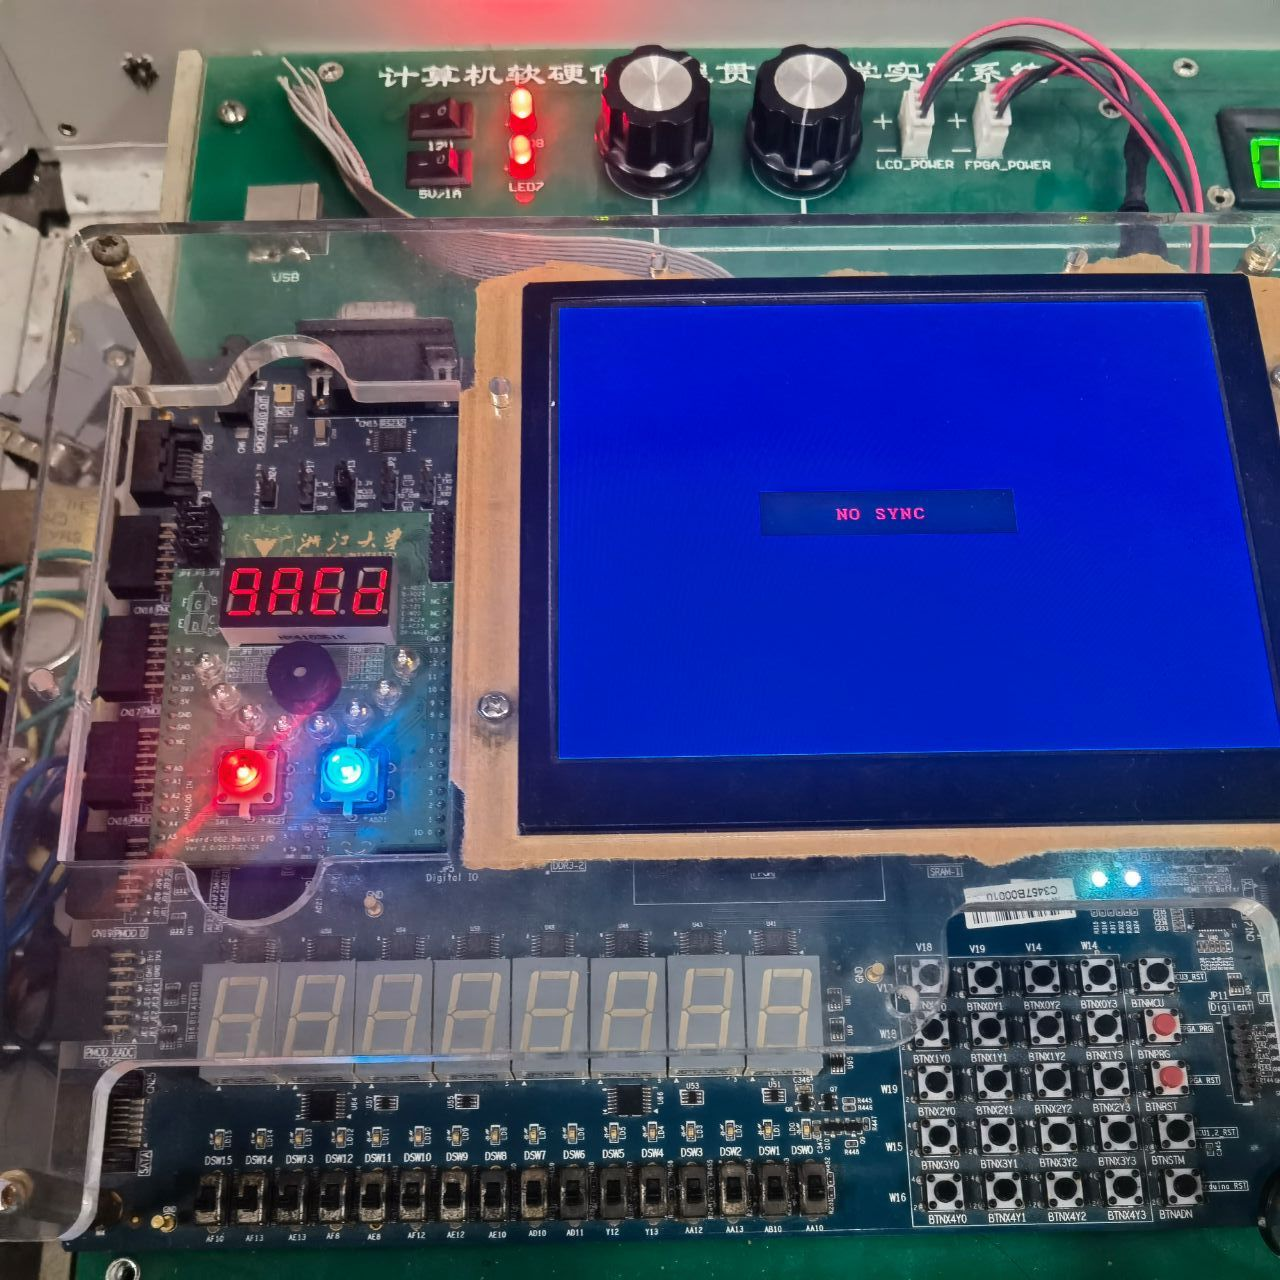
\includegraphics[width=0.4\textwidth]{lab7/10.jpg}
    \caption{\label{Lab7}ScoreBoard下版验证}
    \end{figure}


    \begin{figure}[H]
    \centering
    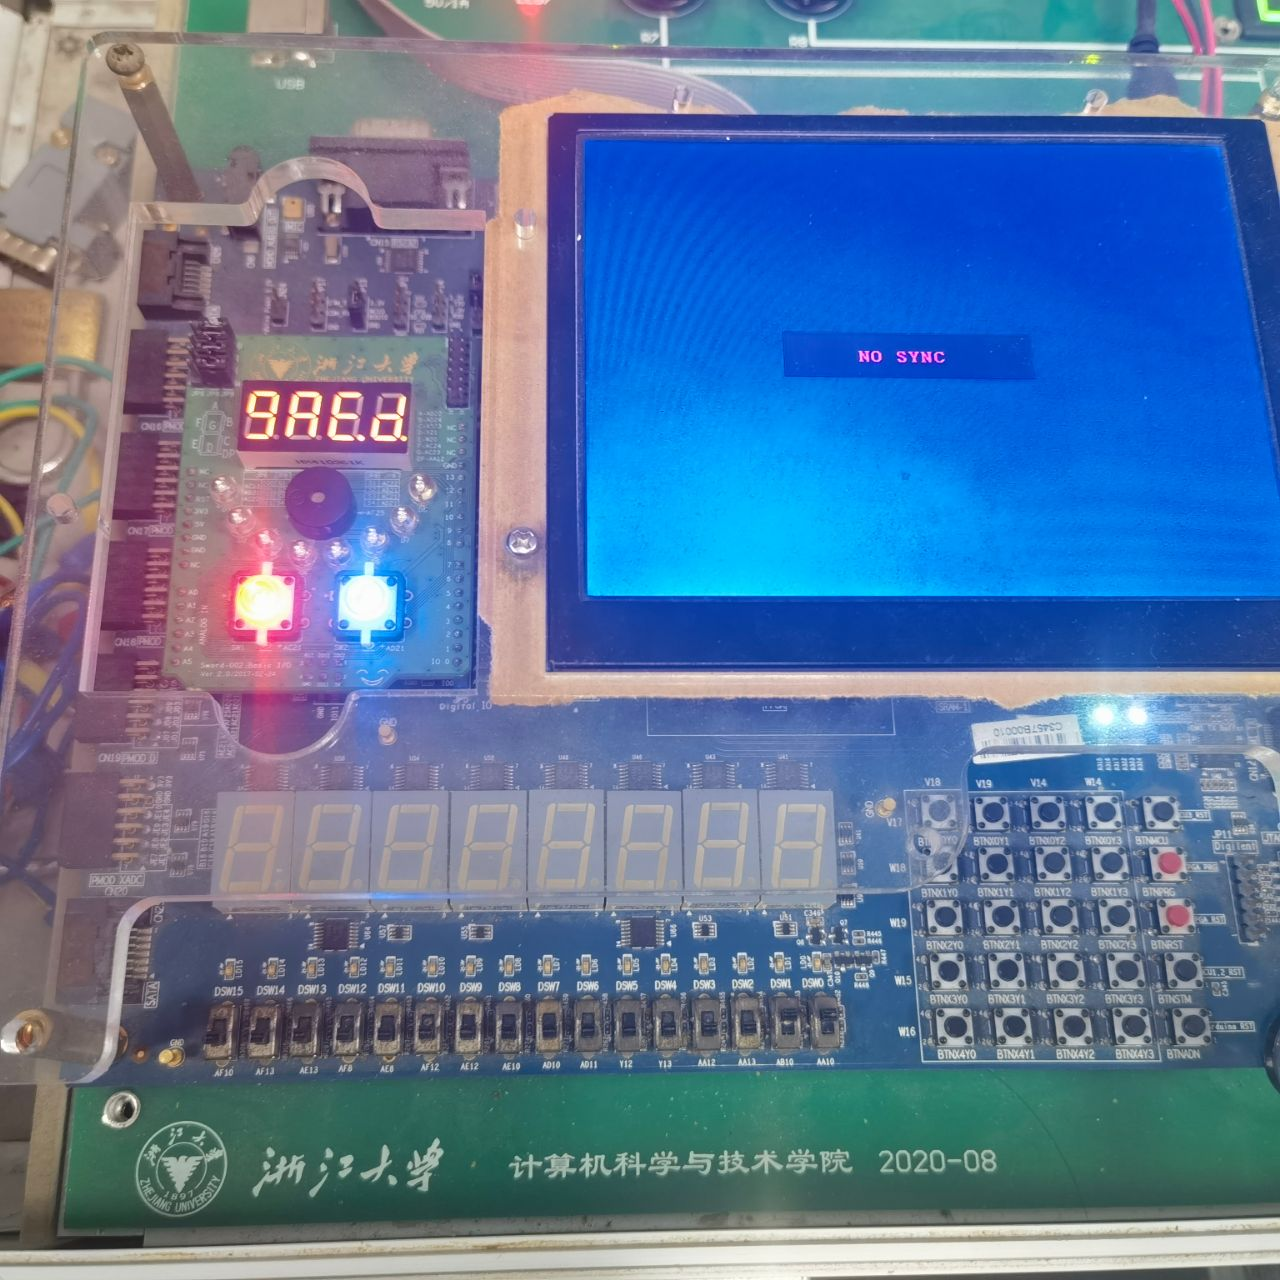
\includegraphics[width=0.4\textwidth]{lab7/11.jpg}
    \caption{\label{Lab7}ScoreBoard下版验证}
    \end{figure}

    \begin{figure}[H]
    \centering
    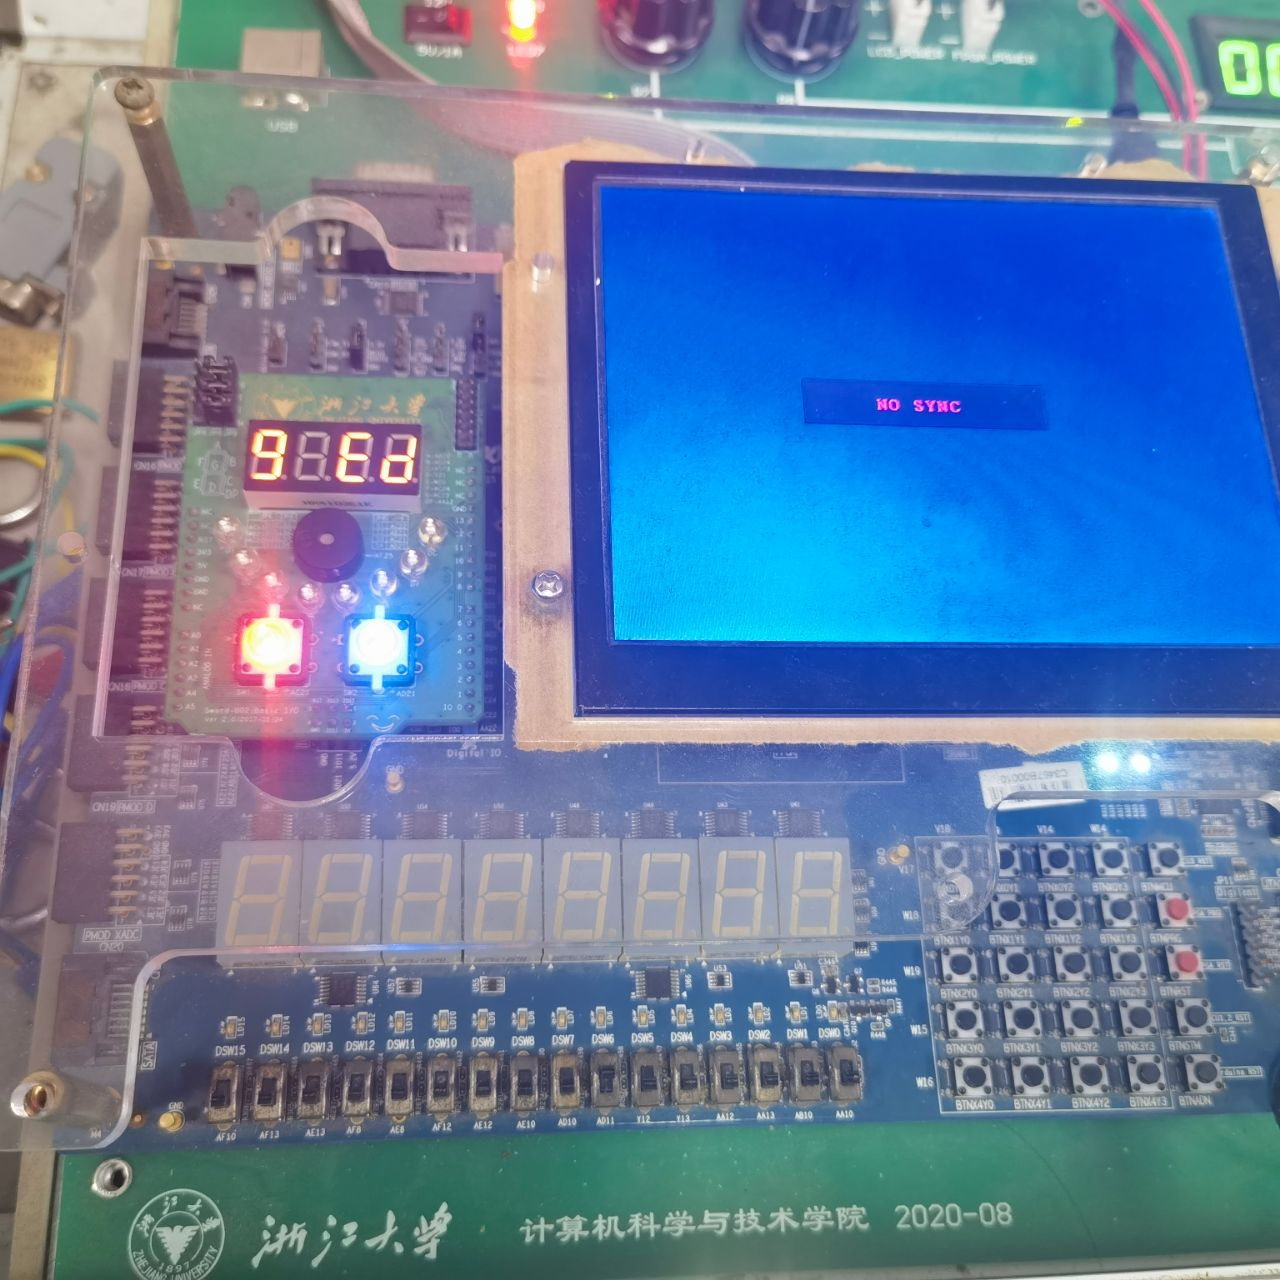
\includegraphics[width=0.4\textwidth]{lab7/12.jpg}
    \caption{\label{Lab7}ScoreBoard下版验证}
    \end{figure}
\subsubsection*{分析}
异步显示数字的原理:clkdiv模块每次时钟信号处于上升沿时,对应的num信号递增1,实验中选取num的(16:17)为作为DisplaySync的选择信号,
选择输出一个对应的七段数码管数字,每次选择输出一个数字,但由于变化的过程时间间隔过短,因此人眼看到时会看到四个显示不同的数字.


数字变化原理:每当一组数码管对应的按键按下时对应的数字会增加(由于信号抖动的原因,增加的数值会大于1),当按钮按下时,top.v中调用的
CreateNumber模块会使对应的数码管的数字增加1,从而使显示模块显示的数字增加,但由于没有进行防抖动的处理,信号检测时会认为信号的变化
不止一次,因此会造成多次增加.


开关控制原理:当LES(3:0)所对应的四个开关被拨动时,对应的数字不会显示,在模块中,LES(3:0)的四个信号分别对应四组数码管的使能信号,
如果使能信号处于关闭状态时,那么对应的数码管便不会显示,在总的模块中LES(3:0)是对应数码管的控制,AN(3:0)对应的是clk信号的控制.
points(3:0)所对应的开关控制了小数点部分的亮暗,它的控制原理和LES(3:0)的控制原理是类似的.

\section{讨论与心得}
本次实验遇到的主要问题是:(1)在DisPlaySync的原理图绘制时,MUX对应的四个输入信号在模块中不是按照递增顺序给出的,在连入对应的输入
信号时,没有看清对应的关系,导致有两部分对应的信号连接反了,导致开关控制时,有两个开关对应的控制数码管弄反,问题就在于此.
(2)绘制完一位MUX之后直接在此基础上绘制了四位MUX,没有对一位MUX进行保存,而后续实验又再次用到了一位MUX,重新进行的重复的绘制.

\end{document}